\section{Results and Discussion}
\label{sec:results}

\subsection{Physical Parametric Trends}
\label{subsec:physical_trends}

Before turning to the surrogate models, the raw CFD dataset itself is examined directly for the effect of each of the four inputs on $Nu$, one at a time, at a fixed representative geometry and operating point (Figure~\ref{fig:sensitivity}). This is a direct property of the CFD solutions, distinct from the SHAP-based interpretability of the trained surrogate reported below: SHAP characterizes what the model learned, whereas the trends here are read directly off the dataset with no model in between.

Figures~\ref{fig:sensitivity}a-b show $Nu$ against $Re$ and $Ri$ respectively, at the concentric $R^\ast=0.3$ geometry, each panel holding the other of the two at three representative levels. At fixed $Ri=0.01$ (rotation-dominated, weak relative buoyancy), $Nu$ is essentially flat across the full $Re=10$-to-$1000$ range ($5.522\to5.550$, a $0.5\%$ change); at fixed $Ri=10$ (buoyancy-dominated), the same $Re$ range produces a $329\%$ increase ($5.523\to23.711$). Symmetrically, at fixed $Re=10$, $Ri$ has almost no effect ($5.522\to5.523$ from $Ri=0.01$ to $10$), while at fixed $Re=1000$ the same $Ri$ range produces a $327\%$ increase. Because $Ra=0.71\,Ri\,Re^2$, holding either $Re$ or $Ri$ fixed while sweeping the other still changes the achieved Rayleigh number along that curve; the pattern above is consistent with $Nu$ tracking the achieved $Ra$ more directly than either $Re$ or $Ri$ in isolation, with $Re$ and $Ri$ acting as the two control variables that jointly set it. This is also consistent with the SHAP ranking reported below, where $Re$'s larger mean impact partly reflects its role in amplifying $Ri$'s effect (evident in Figure~\ref{fig:sensitivity}a's fan of curves) rather than a large effect at every fixed $Ri$.

Figure~\ref{fig:sensitivity}c shows $Nu$ against $R^\ast$ across the six concentric geometries at a fixed operating point ($Re=125$, $Ri=1$): the trend is non-monotonic, falling from $9.877$ at $R^\ast=0.1$ to a minimum of $5.488$ at $R^\ast=0.4$ before rising again to $6.520$ at $R^\ast=0.6$. Because the $Nu=q''/k$ convention used throughout this dataset is not normalized to the pure-conduction limit, as noted above, part of this trend reflects the purely geometric conduction shape factor $S$, Equation~\eqref{eq:shape-factor}, which itself grows sharply as $R^\ast\to0$ independent of any convective effect; the classical-convention conversion given above is the appropriate lens for isolating the convective radius-ratio effect specifically, and this raw-$Nu$ panel should be read as a property of the achieved heat flux, not of convective strength alone. Figure~\ref{fig:sensitivity}d shows $Nu$ against eccentricity within the $R^\ast=0.3$ group at the same operating point, increasing monotonically and smoothly by $18.3\%$ from the concentric case to the group's maximum eccentricity, consistent with the positive eccentricity effect recovered independently by the trained surrogate's SHAP analysis below.

\begin{figure}[h]
\centering
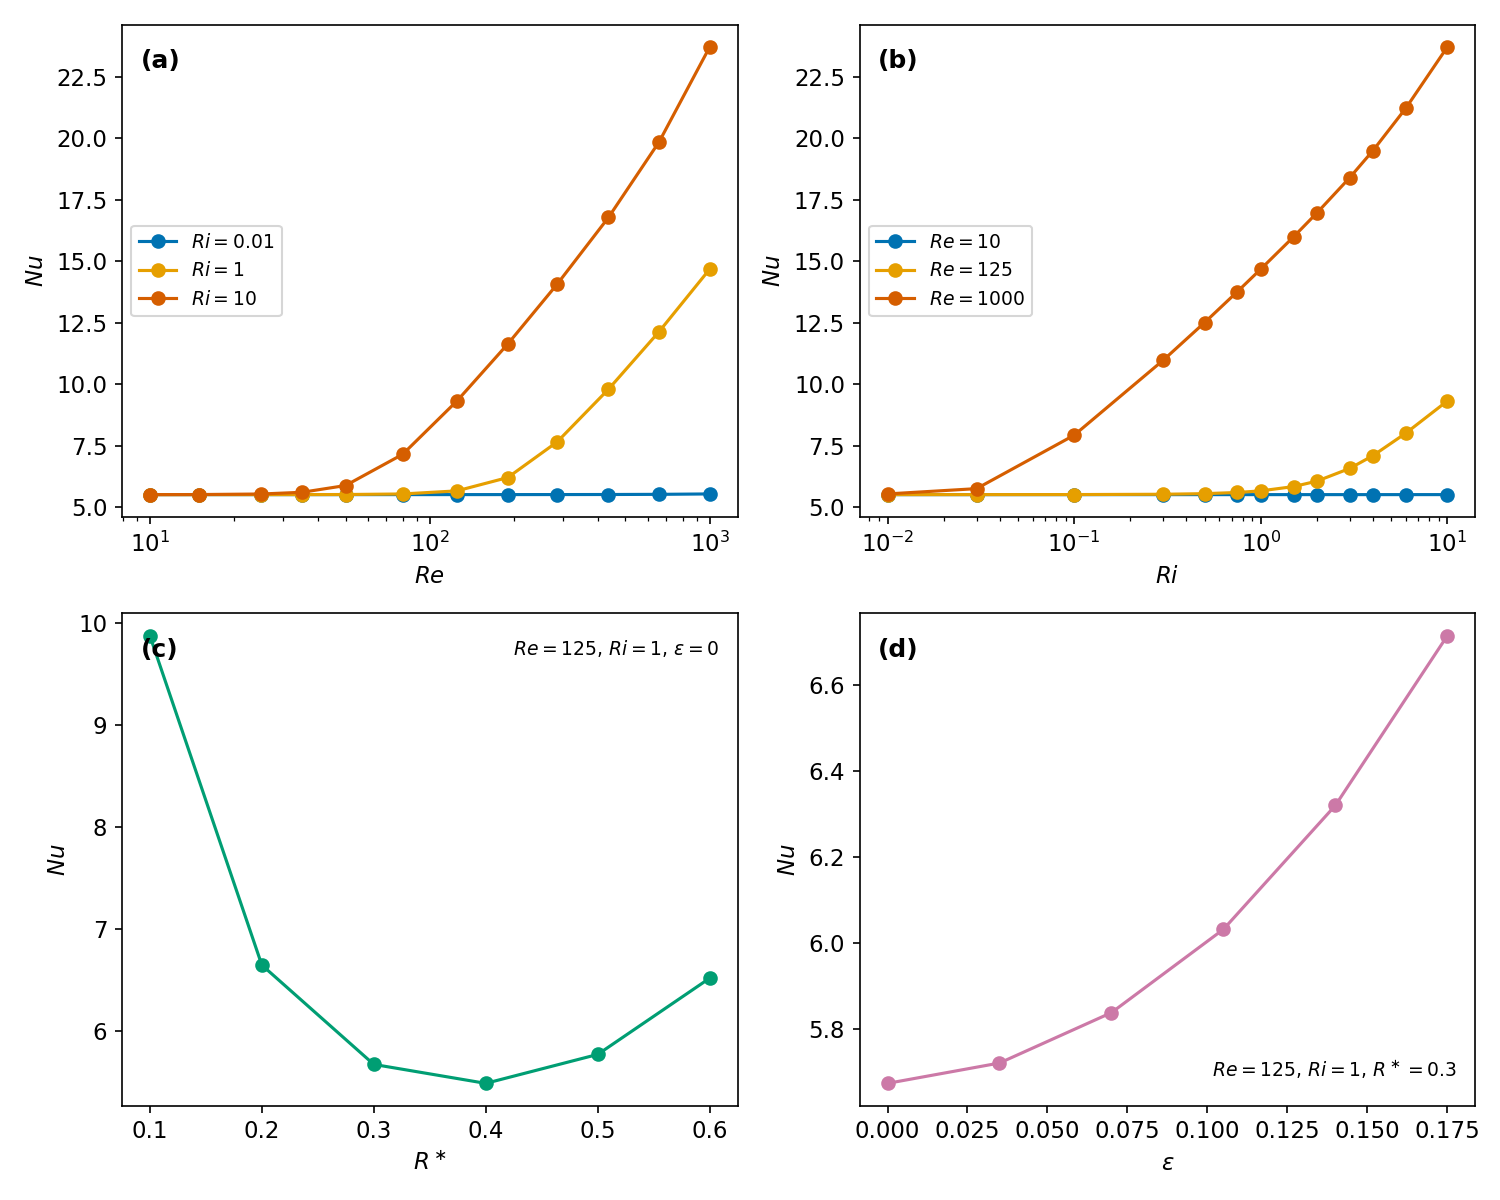
\includegraphics[width=\textwidth]{figures/fig_sensitivity.png}
\caption{Physical parametric trends read directly from the CFD dataset. (a) $Nu$ vs.\ $Re$ at $R^\ast=0.3$, $\varepsilon=0$, for three fixed $Ri$. (b) $Nu$ vs.\ $Ri$ at the same geometry, for three fixed $Re$. (c) $Nu$ vs.\ $R^\ast$ across the six concentric geometries at $Re=125$, $Ri=1$. (d) $Nu$ vs.\ $\varepsilon$ within the $R^\ast=0.3$ group at the same operating point.}
\label{fig:sensitivity}
\end{figure}

\subsection{Scalar Nusselt Number Surrogate}
\label{subsec:scalar_results}

Table~\ref{tab:scalar-bakeoff} and Figure~\ref{fig:scalar-bakeoff} report the same-grid 70/30 holdout performance of the three candidate architectures ($n=1{,}638$ held-out test rows). XGBoost achieves the highest accuracy on every metric, followed by the physics-informed neural network, with the Kolmogorov-Arnold Network trailing on both metrics.

\begin{table}[h]
\centering
\caption{Scalar Nusselt number surrogate comparison, same-grid 70/30 test split.}
\label{tab:scalar-bakeoff}
\begin{tabular}{lccc}
\toprule
Model & Test $R^2$ & Test MAPE (\%) & Test RMSE \\
\midrule
XGBoost & 0.99963 & 0.64 & 0.099 \\
PINN & 0.99936 & 1.07 & 0.132 \\
KAN & 0.99725 & 2.17 & 0.272 \\
\bottomrule
\end{tabular}
\end{table}

\begin{figure}[h]
\centering
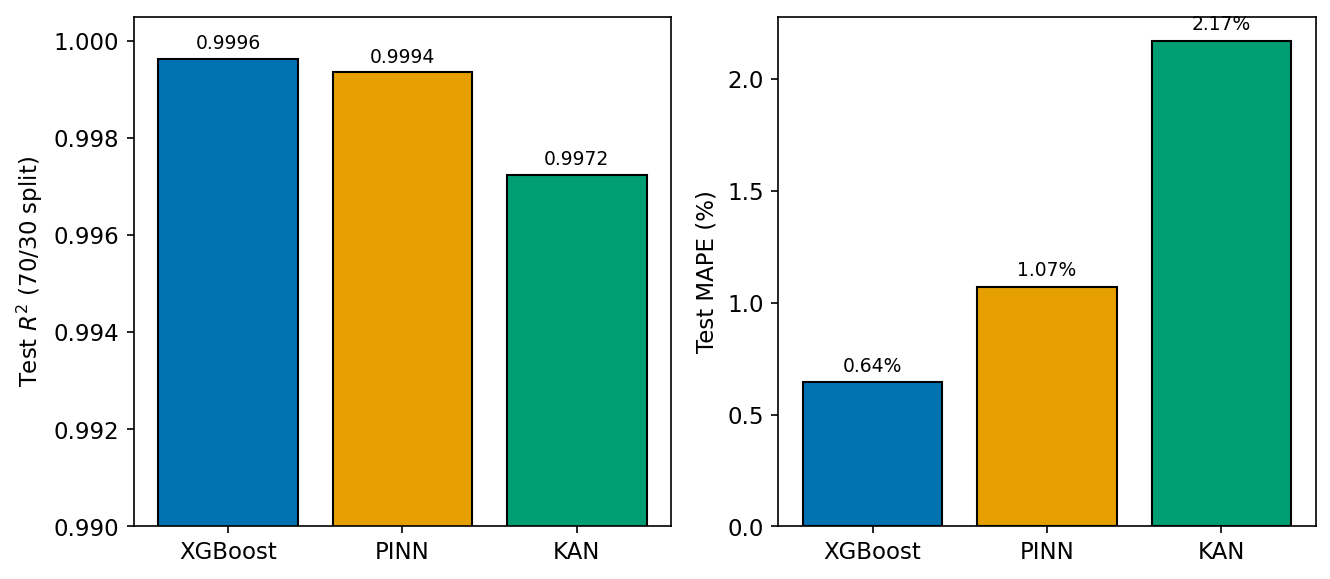
\includegraphics[width=\textwidth]{figures/fig_scalar_bakeoff.png}
\caption{Scalar Nusselt number surrogate comparison, same-grid 70/30 test split.}
\label{fig:scalar-bakeoff}
\end{figure}

The near-unity test-set $R^2$ reflects the noise-free, deterministic nature of the CFD data and the same-grid split's interpolative character, between $(Re,Ri)$ values already present in the sampling grid; Section~\ref{subsec:oos} shows this figure does not hold under genuine extrapolation.

Because the 70/30 split draws test points from geometries also represented in training, a stricter test was run: 35-fold Leave-One-Geometry-Out (LOGO) cross-validation, in which the model is retrained 35 times, each time withholding all rows for one distinct $(R^\ast,\varepsilon)$ combination entirely. This measures generalization across the geometric parameter space specifically. Across the 35 folds, mean $R^2 = 0.9977$ (standard deviation $0.0032$, minimum $0.9836$) and mean absolute percentage error $= 1.65\%$ (maximum $5.79\%$). The weakest-performing geometries were consistently found at the high-eccentricity edge of their radius ratio's sampled range ($R^\ast=0.1,\varepsilon=0.315$: $R^2=0.9836$, MAPE $5.79\%$; $R^\ast=0.2,\varepsilon=0.24$: $R^2=0.9912$, MAPE $4.65\%$), consistent with reduced accuracy at the boundary of the trained parameter space rather than a systematic modeling failure.

\subsubsection{True Out-of-Sample Validation}
\label{subsec:oos}

The metrics above, including the LOGO result, are computed on $(Re,Ri)$ combinations that were themselves part of the original 5,460-case sampling grid, even when the specific geometry or row was held out. To measure genuine extrapolation accuracy, eighteen additional numerical simulations were run at $(Re,Ri)$ combinations constructed to fall strictly between the grid points used to generate the training data, at six of the thirty-five existing mesh geometries. All eighteen converged. An initial set of twelve such points, chosen without regard to the resulting $Nu$ they would produce, left an unintended gap in achieved Rayleigh number between $Ra\approx2.7\times10^5$ and $Ra\approx2.3\times10^6$; six further points were added specifically to fill that gap, log-uniformly in $Ra$, so that the extrapolation test spans the achieved output range rather than clustering at its low end by accident.

Across these eighteen points, the mean absolute error is $7.89\%$ (median $5.83\%$, maximum $23.33\%$), a materially higher and more representative figure than the $0.64\%$ same-grid test error above, and higher than the $5.92\%$ figure an evaluation on only the original twelve points would have reported: the gap-filling points expose real extrapolation error that the initial, accidentally low-$Ra$-clustered set understated. Figure~\ref{fig:blind-parity} shows predicted against true values for these eighteen points (left) and the absolute percentage error at each point, sorted by Nusselt number (right); the thin gray connectors in the left panel show each point's vertical deviation from perfect prediction. The seven points at $Re \leq 150$ show error at or below $4.95\%$ (mean $0.98\%$); the eleven points at $Re \geq 300$ show substantially higher and more variable error (mean $12.3\%$, range $3.7$--$23.3\%$), consistent with $Re \geq 300$ being the sparser half of the twelve-value training grid in absolute terms (gaps of $150$ to $340$ between adjacent levels, against $5$ to $45$ below $Re=150$), though the correspondence is not perfectly monotonic: the single point at $Re=700$ ($Ri=4.2$) shows only $3.7\%$ error despite its high $Re$, and the point at $Re=150$ ($Ri=1.25$) shows $4.95\%$ despite falling in the otherwise low-error group.

\begin{figure}[h]
\centering
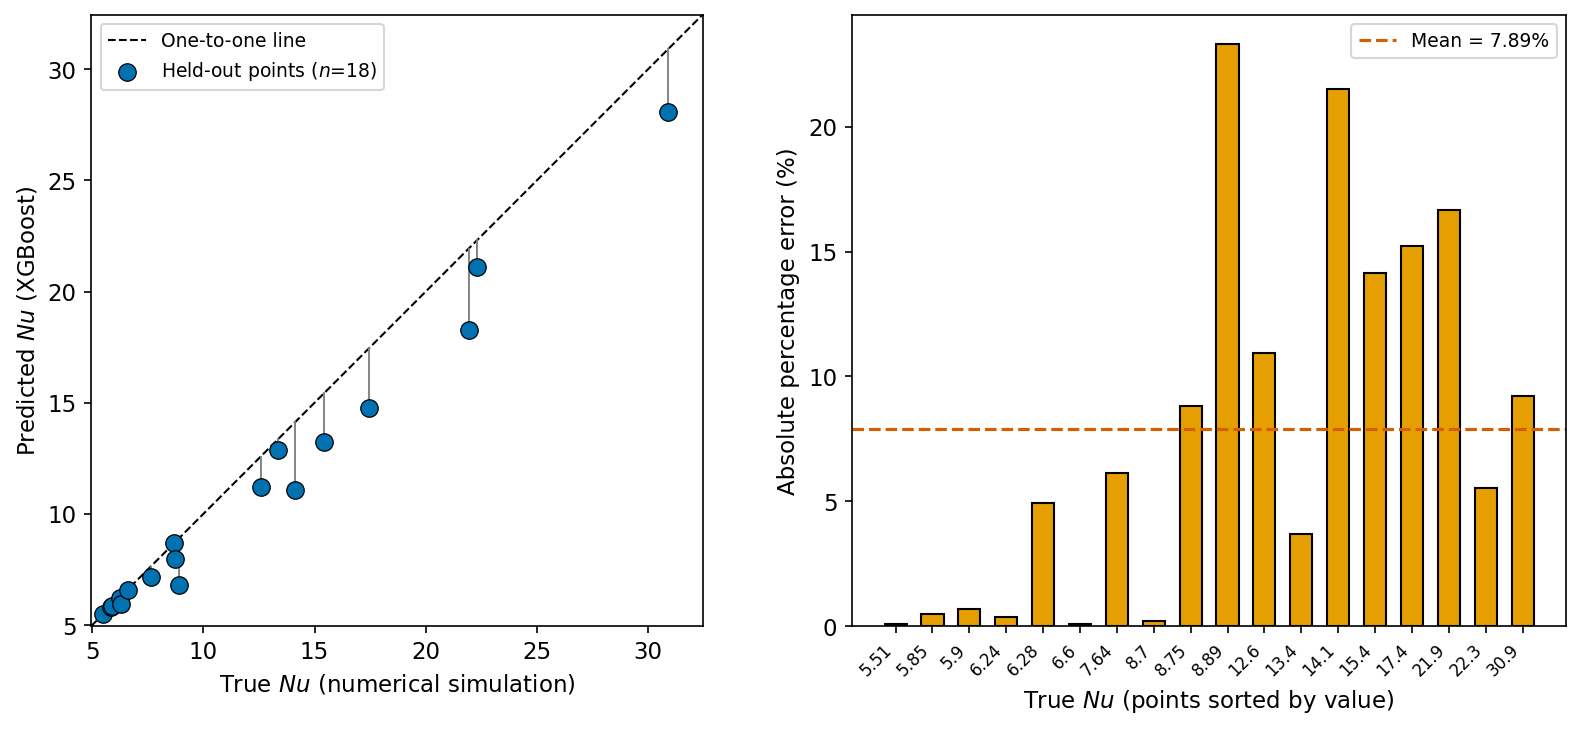
\includegraphics[width=\textwidth]{figures/fig_blind_test_parity.png}
\caption{True out-of-sample test at eighteen numerical simulations run at $(Re,Ri)$ combinations never present in the training data. Left: predicted versus true Nusselt number, with gray connectors showing each point's deviation from the one-to-one line. Right: absolute percentage error per point, sorted by true Nusselt number, with the mean (7.89\%) marked.}
\label{fig:blind-parity}
\end{figure}

Both accuracy figures are reported deliberately: the $0.64\%$ same-grid figure measures interpolation within the sampled grid, and the $7.89\%$ true out-of-sample figure measures genuine predictive accuracy on previously unseen physical conditions. The two are not interchangeable, and the same-grid figure alone would overstate the model's real-world reliability.

This $Re$-specific error pattern raises an immediate question with a direct bearing on how Figure~\ref{fig:blind-parity} should be read: does the increasing error reflect a change in the underlying convection regime, for instance the transition between buoyancy-dominated and rotation-dominated flow controlled by $Ri$, or is it a property of the training grid rather than the physics? The two hypotheses make different, testable predictions. A regime-transition effect would concentrate error near the $Ri\sim1$ mixed-convection transition regardless of $Re$; a grid-resolution effect would track $Re$ specifically, regardless of $Ri$. Across these eighteen points, error correlates far more strongly with $Re$ ($r=0.72$) than with $Ri$ ($r=0.20$), and the two largest errors occur at opposite ends of the $Ri$ range ($Ri=0.2$, rotation-dominated: $23.3\%$; $Ri=3.6$, buoyancy-leaning: $21.5\%$), while an intermediate point at $Ri=4.2$ shows only $3.7\%$ error; error does not concentrate near $Ri\sim1$. The regime-transition hypothesis is not supported by the data.

The $Re$-specific pattern instead has two compounding causes, both properties of the twelve-level $Re$ training grid rather than of the flow physics. First, that grid is log-spaced from $Re=10$ to $1000$ for even coverage in relative terms, but XGBoost splits on the raw $Re$ value, so the absolute gap between neighboring training levels still grows roughly fifty-to-seventy-fold across the sweep (from $5$--$15$ near $Re=10$ to $225$--$340$ near $Re=1000$); the width of the training-grid interval bracketing each blind point correlates with its error at $r=0.66$, the strongest relationship found among all quantities tested, including $Nu$ itself ($r=0.43$). Second, this coarser absolute resolution coincides with the region where $Nu$ responds most steeply to $Re$: Section~\ref{subsec:physical_trends} reports a $329\%$ change in $Nu$ across the full $Re$ sweep at $Ri=10$, against an essentially flat response at $Ri=0.01$; a local-sensitivity proxy, $\partial Ra/\partial Re$ at fixed $Ri$, correlates with error at $r=0.46$. A coarser absolute grid over a steeper local response compounds into larger interpolation error independent of any change in flow regime. Because $Ri$ alone moves $Nu$ by well under $1\%$ at low $Re$ (Section~\ref{subsec:physical_trends}), large-$Nu$ points in this eighteen-point set occur almost exclusively at high $Re$; the apparent growth of error with $Nu$ in Figure~\ref{fig:blind-parity} (right) is therefore inherited from this $Re$-specific effect, not a separate consequence of the output's own magnitude.

\subsubsection{Uncertainty Quantification}
\label{subsec:uq_results}

A 20-member bootstrap ensemble of the winning XGBoost configuration was used to quantify predictive uncertainty. On the same-grid test split, $97.9\%$ of true values fell within the ensemble's own 95\% predictive interval, close to nominal (if anything, slightly over-covered). On the true out-of-sample test set described above, however, only $27.8\%$ of true values fell within the reported 95\% interval (Figure~\ref{fig:uq-calibration}); the ensemble's predictive standard deviation at these points is small relative to the actual errors observed, because bootstrap resampling of the training set captures uncertainty about which training rows were sampled, but does not capture the model's true epistemic uncertainty when extrapolating to $(Re,Ri)$ conditions genuinely absent from the training grid. This is a general property of ensemble-based uncertainty methods, not a flaw specific to the bootstrap approach used here: they quantify sensitivity to the training sample rather than epistemic uncertainty about extrapolation beyond the sampled input distribution.

\begin{figure}[h]
\centering
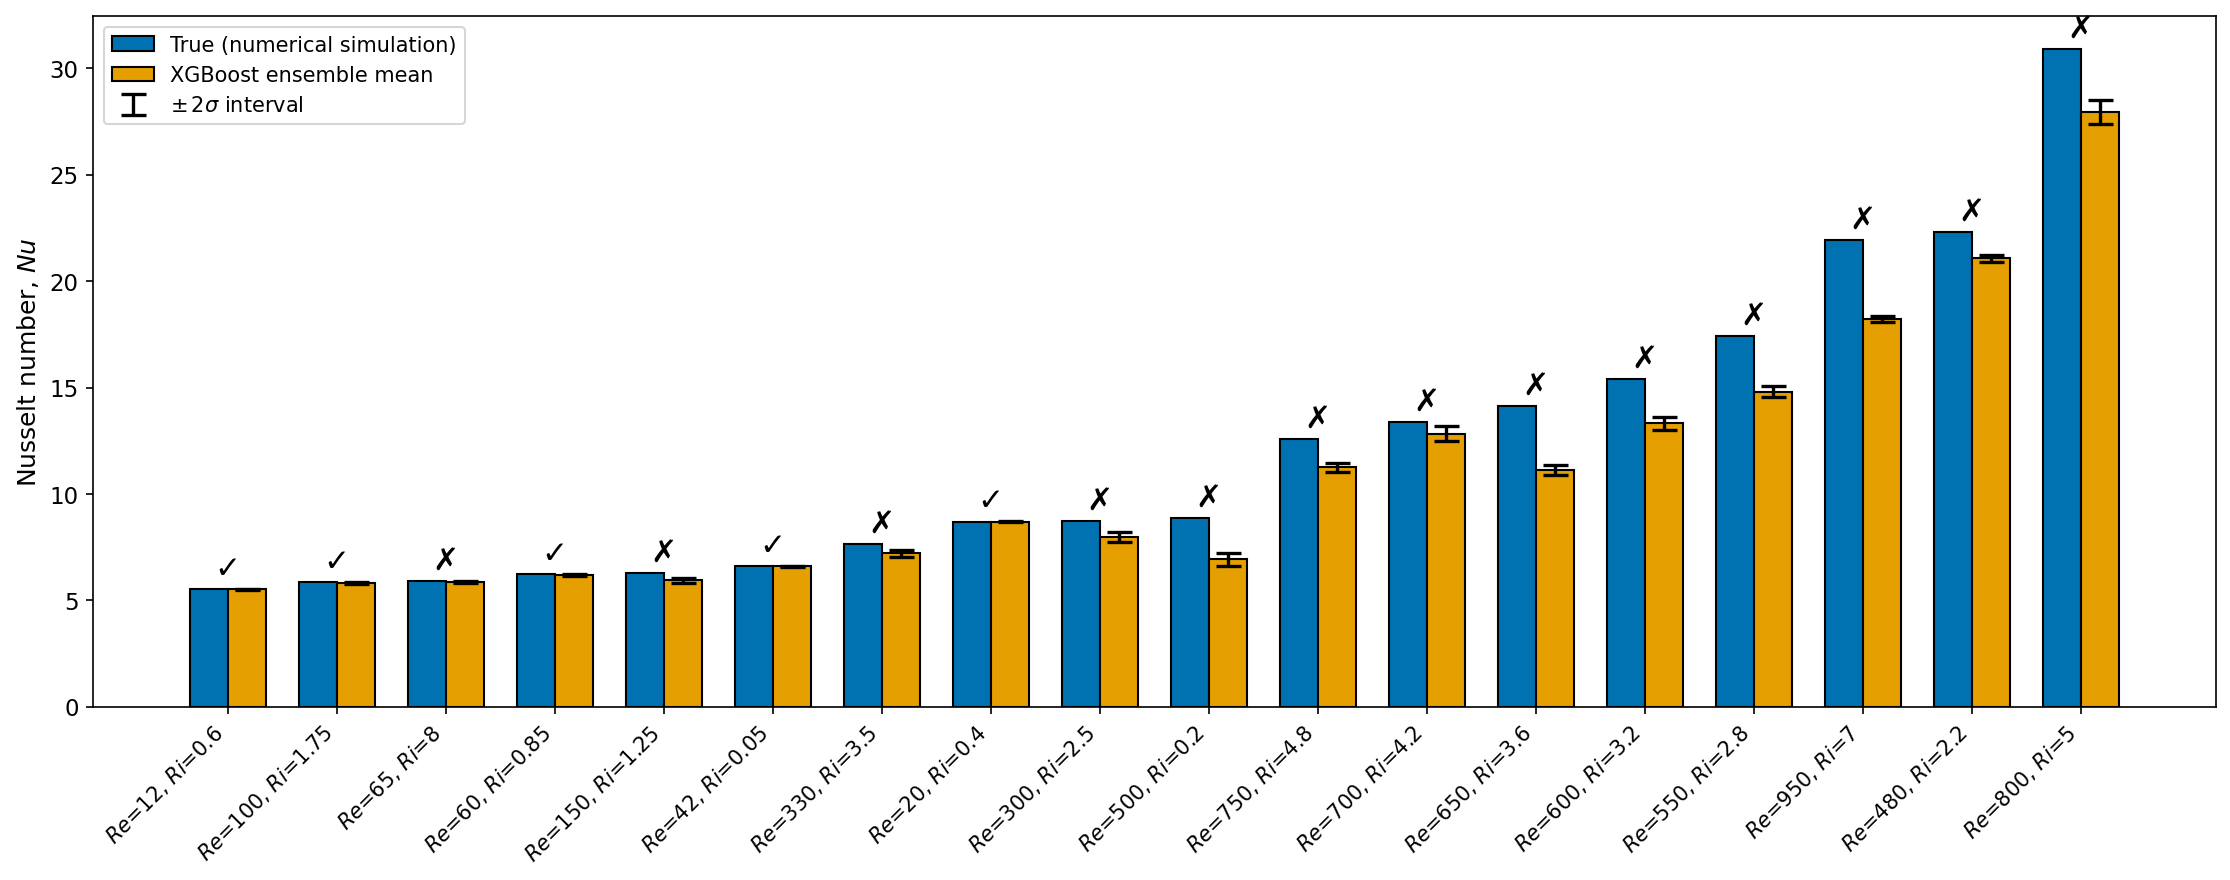
\includegraphics[width=\textwidth]{figures/fig_uq_calibration.png}
\caption{True out-of-sample test: CFD ground truth against the bootstrap ensemble's mean prediction and $\pm 2\sigma$ interval, sorted by Nusselt number. Only $27.8\%$ of points fall within their own reported 95\% interval, against a 95\% target.}
\label{fig:uq-calibration}
\end{figure}

\subsubsection{Interpretability}
\label{subsec:shap_results}

SHAP analysis on the held-out test set ranks input importance as $Re$ ($40\%$) $>$ $R^\ast$ ($32\%$) $>$ $Ri$ ($23\%$) $\gg$ $\varepsilon$ ($5\%$) of total mean $|$SHAP value$|$, consistent with the model's native gain-based feature importance (Section~\ref{subsec:scalar_arch}) and with the effect directions already established in Section~\ref{subsec:physical_trends}.

\subsection{Spatial Field Surrogate}
\label{subsec:field_results}

Table~\ref{tab:field-bakeoff} and Figure~\ref{fig:field-bakeoff} report the case-level (geometry-held-out) test performance of the three spatial-field candidates, evaluated on an identical split of 24 training geometries and 11 entirely held-out test geometries.

\begin{table}[h]
\centering
\caption{Spatial field surrogate comparison, test $R^2$ on 11 held-out geometries.}
\label{tab:field-bakeoff}
\begin{tabular}{lccc}
\toprule
Model & Temperature & $u$ & $v$ \\
\midrule
Per-node MLP & 0.966 & 0.962 & 0.967 \\
GNN (true mesh connectivity) & 0.957 & 0.698 & 0.824 \\
DeepONet & 0.647 & 0.489 & 0.550 \\
\bottomrule
\end{tabular}
\end{table}

\begin{figure}[h]
\centering
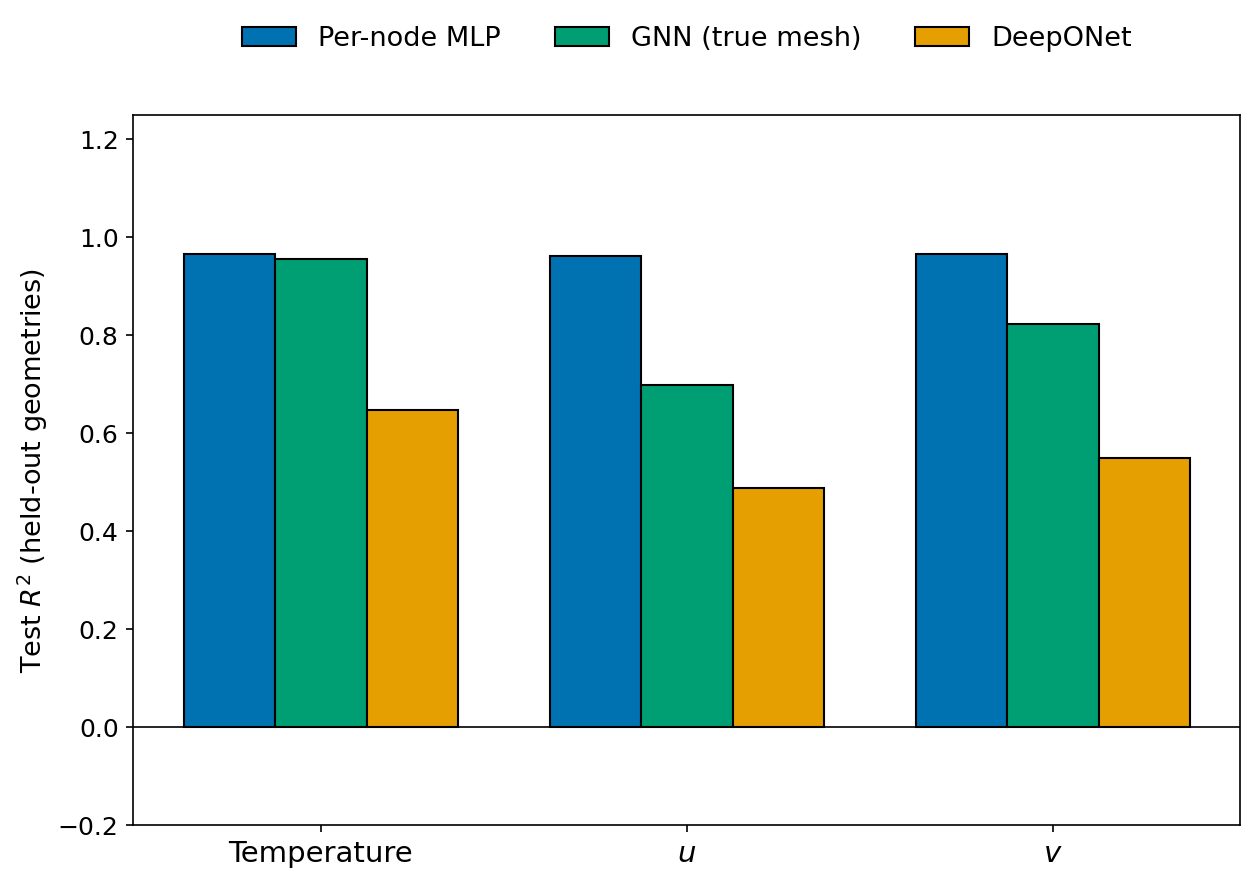
\includegraphics[width=0.95\textwidth]{figures/fig_field_bakeoff.png}
\caption{Spatial field surrogate comparison on 11 held-out geometries.}
\label{fig:field-bakeoff}
\end{figure}

The per-node multilayer perceptron, which conditions each query point directly and jointly on the full case parameters and its own coordinates, outperformed both a DeepONet and a graph neural network using the true finite-volume mesh connectivity, on every target. The DeepONet reached only $R^2=0.49$--$0.65$ across the three targets; the graph neural network matched the per-node MLP closely on temperature ($R^2=0.957$ vs.\ $0.966$) but fell well short on the velocity components ($R^2=0.698$ and $0.824$ for $u$ and $v$, against $0.962$ and $0.967$). This is the same qualitative ranking, per-node MLP ahead of GNN ahead of DeepONet, found under the initial Rayleigh-number/rotation-rate parameterization of this study, obtained here on an independently regenerated dataset with a different underlying physical sweep, which strengthens confidence that the ranking reflects a genuine architectural property of this flow class rather than an artifact of one particular dataset.

This ranking runs counter to the intuition that an architecture aware of the domain's actual topology should have an advantage. Two explanations are consistent with the observed behavior. First, the per-node network conditions every query point directly and simultaneously on the full set of case parameters and its own spatial coordinate, while the graph neural network must propagate information about boundary conditions on the far side of the domain across a limited number of message-passing hops; for a flow in which the whole domain responds coherently to global buoyancy and rotation parameters, this relay delay appears to cost more accuracy than the topological awareness gains. This limitation is consistent with Travnikov et al.~\cite{Travnikov2024}, who document an analogous accuracy degradation for graph neural network surrogates on larger computational domains, attributed to the same limited receptive field of standard message-passing architectures. Second, the DeepONet's characteristic bilinear structure, a dot product between a case-parameter encoding and a coordinate encoding, is a strong architectural assumption that the geometry-and-rotation dependence and the spatial dependence combine in a low-rank, separable way; the near-wall boundary-layer and rotational-shear structure in this flow likely requires a genuinely joint, non-separable interaction between position and the governing parameters, which the per-node network's fully connected structure permits but the DeepONet's factored form does not. Both findings should be read as evidence about this specific globally coupled, rotating buoyant flow, not as a general claim that graph- or operator-based architectures are inferior for spatial surrogate modeling.

\subsubsection{Isotherm and Velocity Field Comparison}
\label{subsec:field_viz}

Figures~\ref{fig:field-temperature} and~\ref{fig:field-velocity} present a direct visual comparison between the CFD ground truth and the per-node MLP surrogate prediction across four held-out test geometries, never seen during training, spanning both radius ratio and eccentricity ($R^\ast=0.2,\varepsilon=0$; $R^\ast=0.2,\varepsilon=0.20$; $R^\ast=0.4,\varepsilon=0$; $R^\ast=0.5,\varepsilon=0.06$), at a common representative operating point ($Re=125$, $Ri=1$). Testing multiple geometries side by side, rather than a single case, is the relevant demonstration here: the surrogate's central claim is generalization across the geometric parameter space, and Figures~\ref{fig:field-temperature} and~\ref{fig:field-velocity} show this directly rather than through a single example. The surrogate reproduces the thermal boundary layer around the heated inner cylinder, its distortion under eccentricity, and the near-wall velocity shear layer at every geometry shown. Figure~\ref{fig:field-difference} shows the corresponding signed difference fields (surrogate minus CFD); errors are small and spatially diffuse over most of the domain, with the largest deviations concentrated near the inner wall and, for the eccentric case, on the narrow side of the gap, consistent with the field-level $R^2$ values in Table~\ref{tab:field-bakeoff} and with the velocity components being harder to reconstruct than temperature.

\begin{figure}[p]
\centering
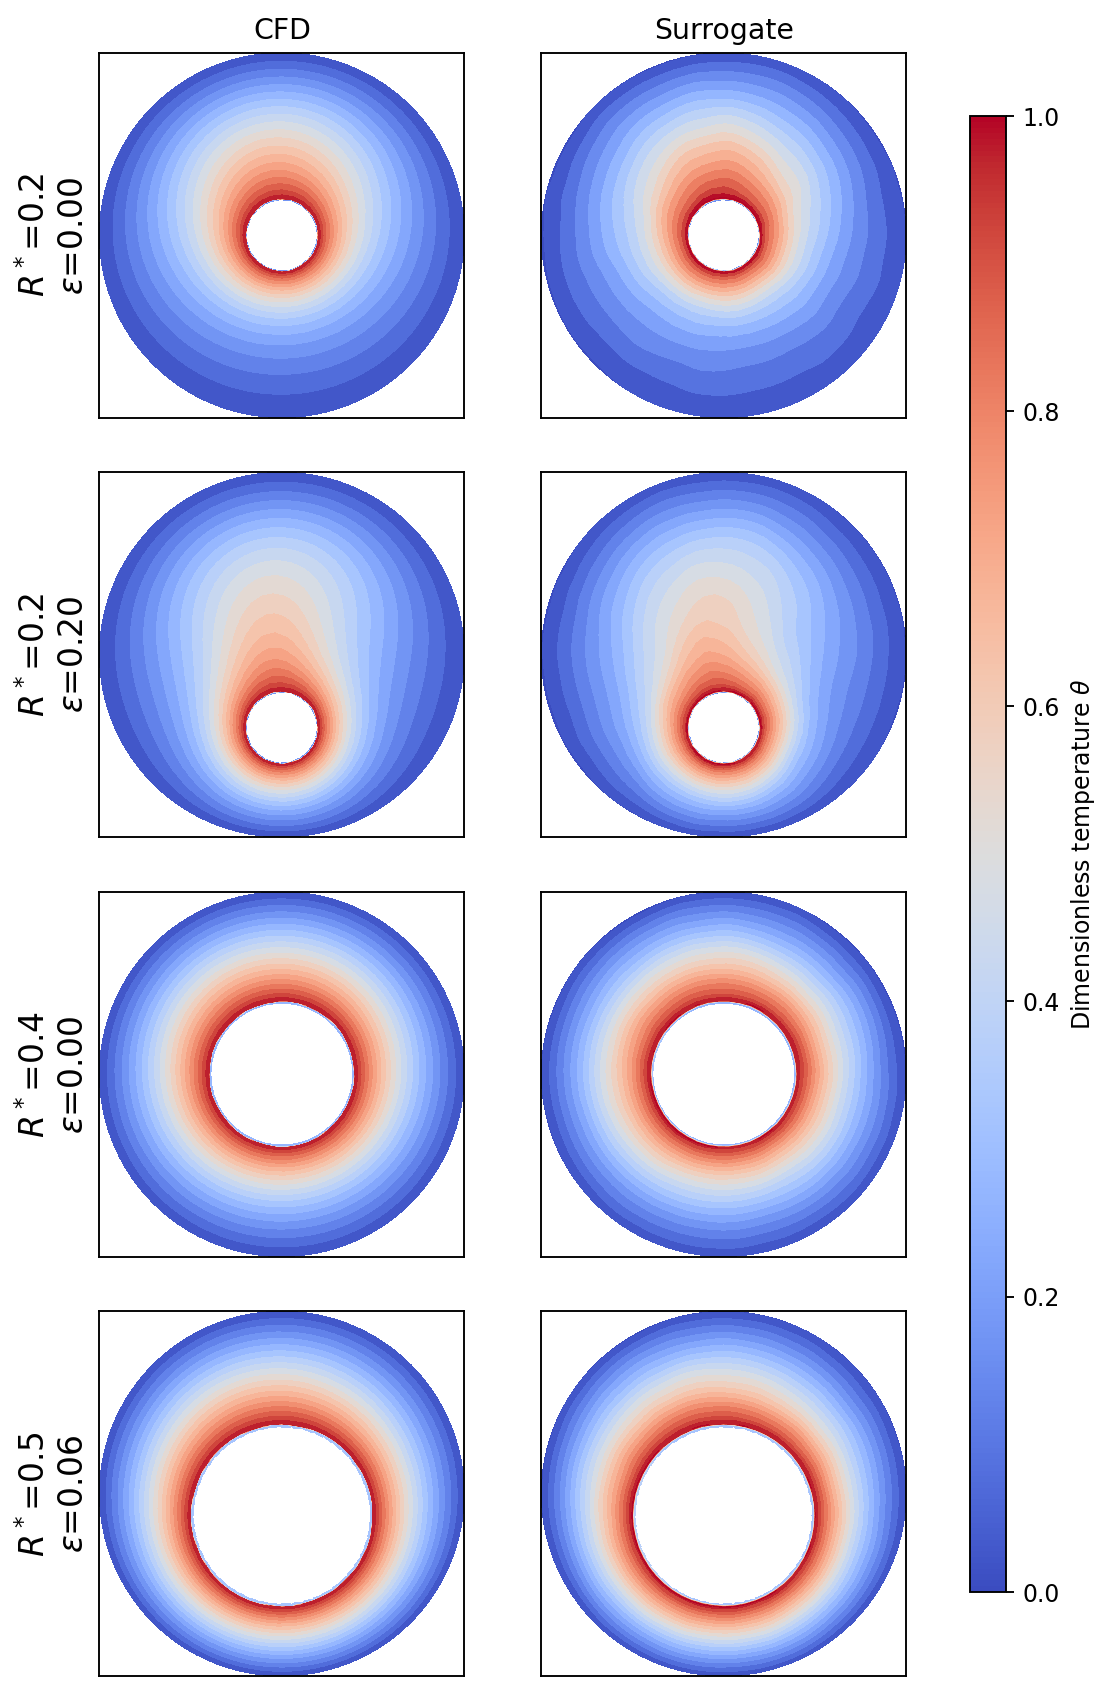
\includegraphics[width=0.7\textwidth]{figures/fig_field_temperature.png}
\caption{CFD ground truth (left) versus per-node MLP surrogate prediction (right) for the dimensionless temperature field, across four held-out test geometries at $Re=125$, $Ri=1$.}
\label{fig:field-temperature}
\end{figure}

\begin{figure}[p]
\centering
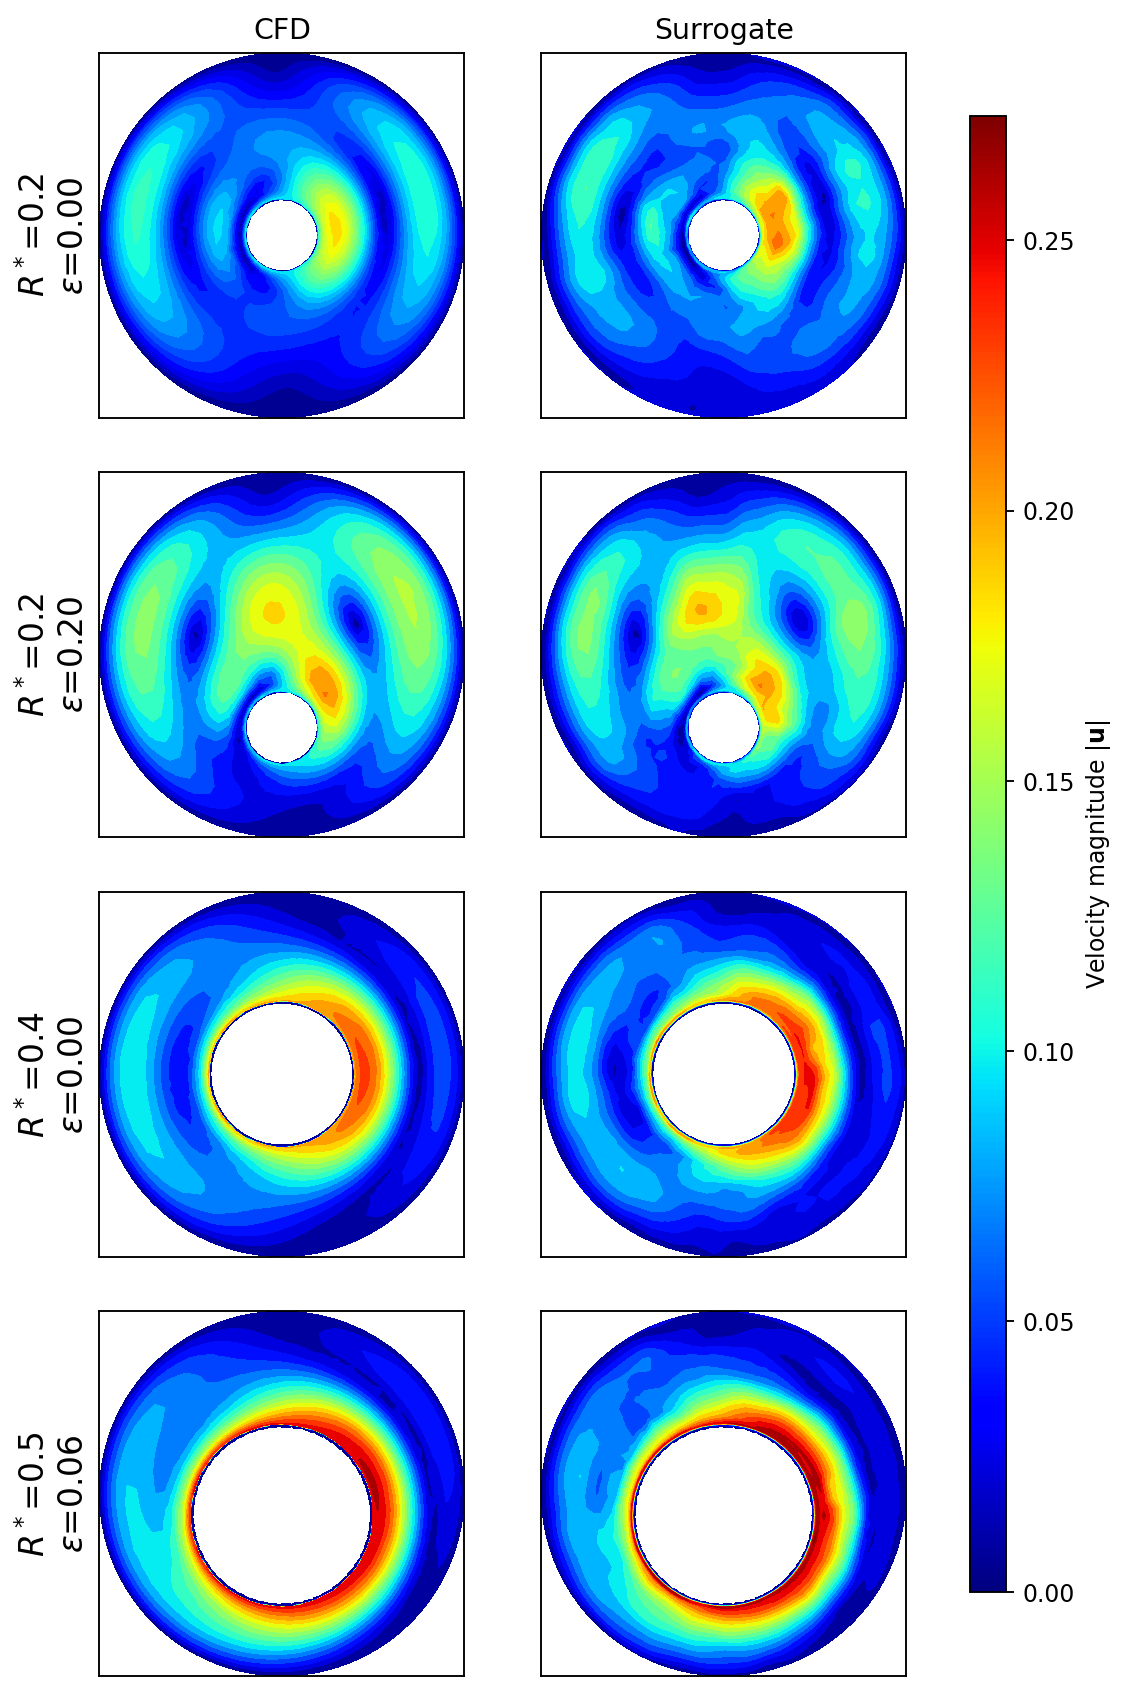
\includegraphics[width=0.7\textwidth]{figures/fig_field_velocity.png}
\caption{CFD ground truth (left) versus per-node MLP surrogate prediction (right) for the velocity magnitude field, across the same four held-out test geometries and operating point as Figure~\ref{fig:field-temperature}.}
\label{fig:field-velocity}
\end{figure}

\begin{figure}[p]
\centering
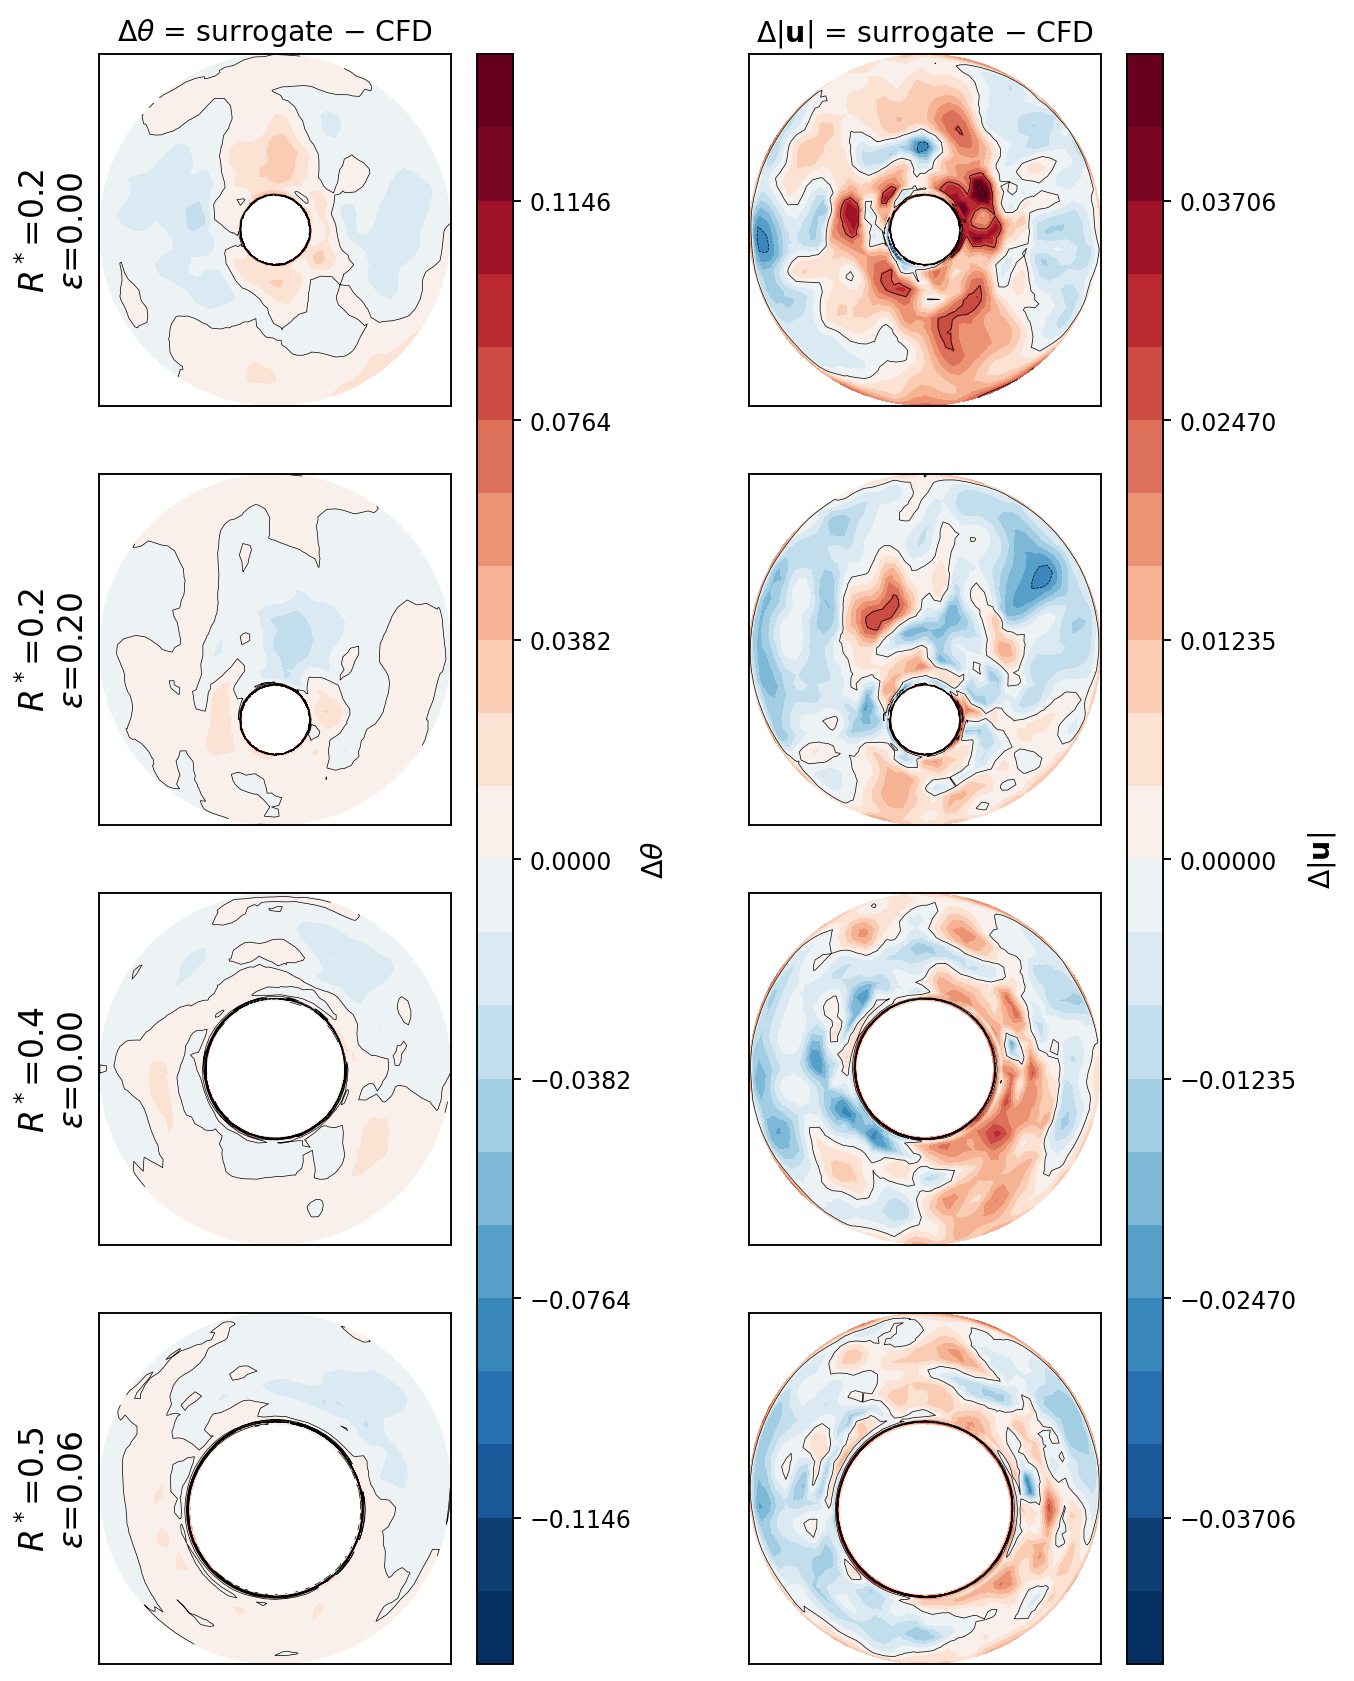
\includegraphics[width=0.7\textwidth]{figures/fig_field_difference.png}
\caption{Signed difference (surrogate minus CFD) for temperature (left) and velocity magnitude (right), for the same four geometries and operating point as Figures~\ref{fig:field-temperature} and~\ref{fig:field-velocity}. Both quantities are differences of already non-dimensional fields and are themselves dimensionless. Contour lines mark equal-difference levels; the color scale is clipped at the 98th percentile of the pooled absolute difference (arrows on the color bar) so that the small fraction of near-boundary outlier nodes does not wash out the contrast in the bulk of the field, where agreement is close.}
\label{fig:field-difference}
\end{figure}

\subsubsection{Out-of-Range Field Validation}
\label{subsec:field_oor}

The scalar surrogate's true out-of-sample test described above was extended to the spatial field surrogate with one additional CFD simulation, including full nodal field export, at a $(Re,Ri)$ combination absent from the training grid ($Re=500$, $Ri=0.2$, at held-out geometry $R^\ast=0.2$, $\varepsilon=0.04$, case 10). This point was chosen deliberately, not for a favorable result: it is one of the eighteen scalar blind-test points above, and specifically the one with the largest scalar surrogate error ($23.33\%$), so this field check honestly probes the same known-difficult, sparse-grid region of the input space rather than a comfortable one. Figure~\ref{fig:oor-field} compares the resulting CFD field directly against the per-node MLP surrogate's prediction at the same points. The mean absolute error is $0.0147$ for temperature and $0.0091$ for velocity magnitude, both within the same-grid field-level accuracy reported in Table~\ref{tab:field-bakeoff} despite the point's known difficulty for the scalar surrogate, and the surrogate reproduces the thermal plume above the inner cylinder and the rotation-driven velocity concentration with no visually obvious degradation relative to the in-grid comparisons of Figures~\ref{fig:field-temperature} and~\ref{fig:field-velocity}. This is a single case, not a systematic out-of-sample study of the kind performed for the scalar surrogate above; a larger, systematically designed out-of-range field test remains an item for future work.

\begin{figure}[p]
\centering
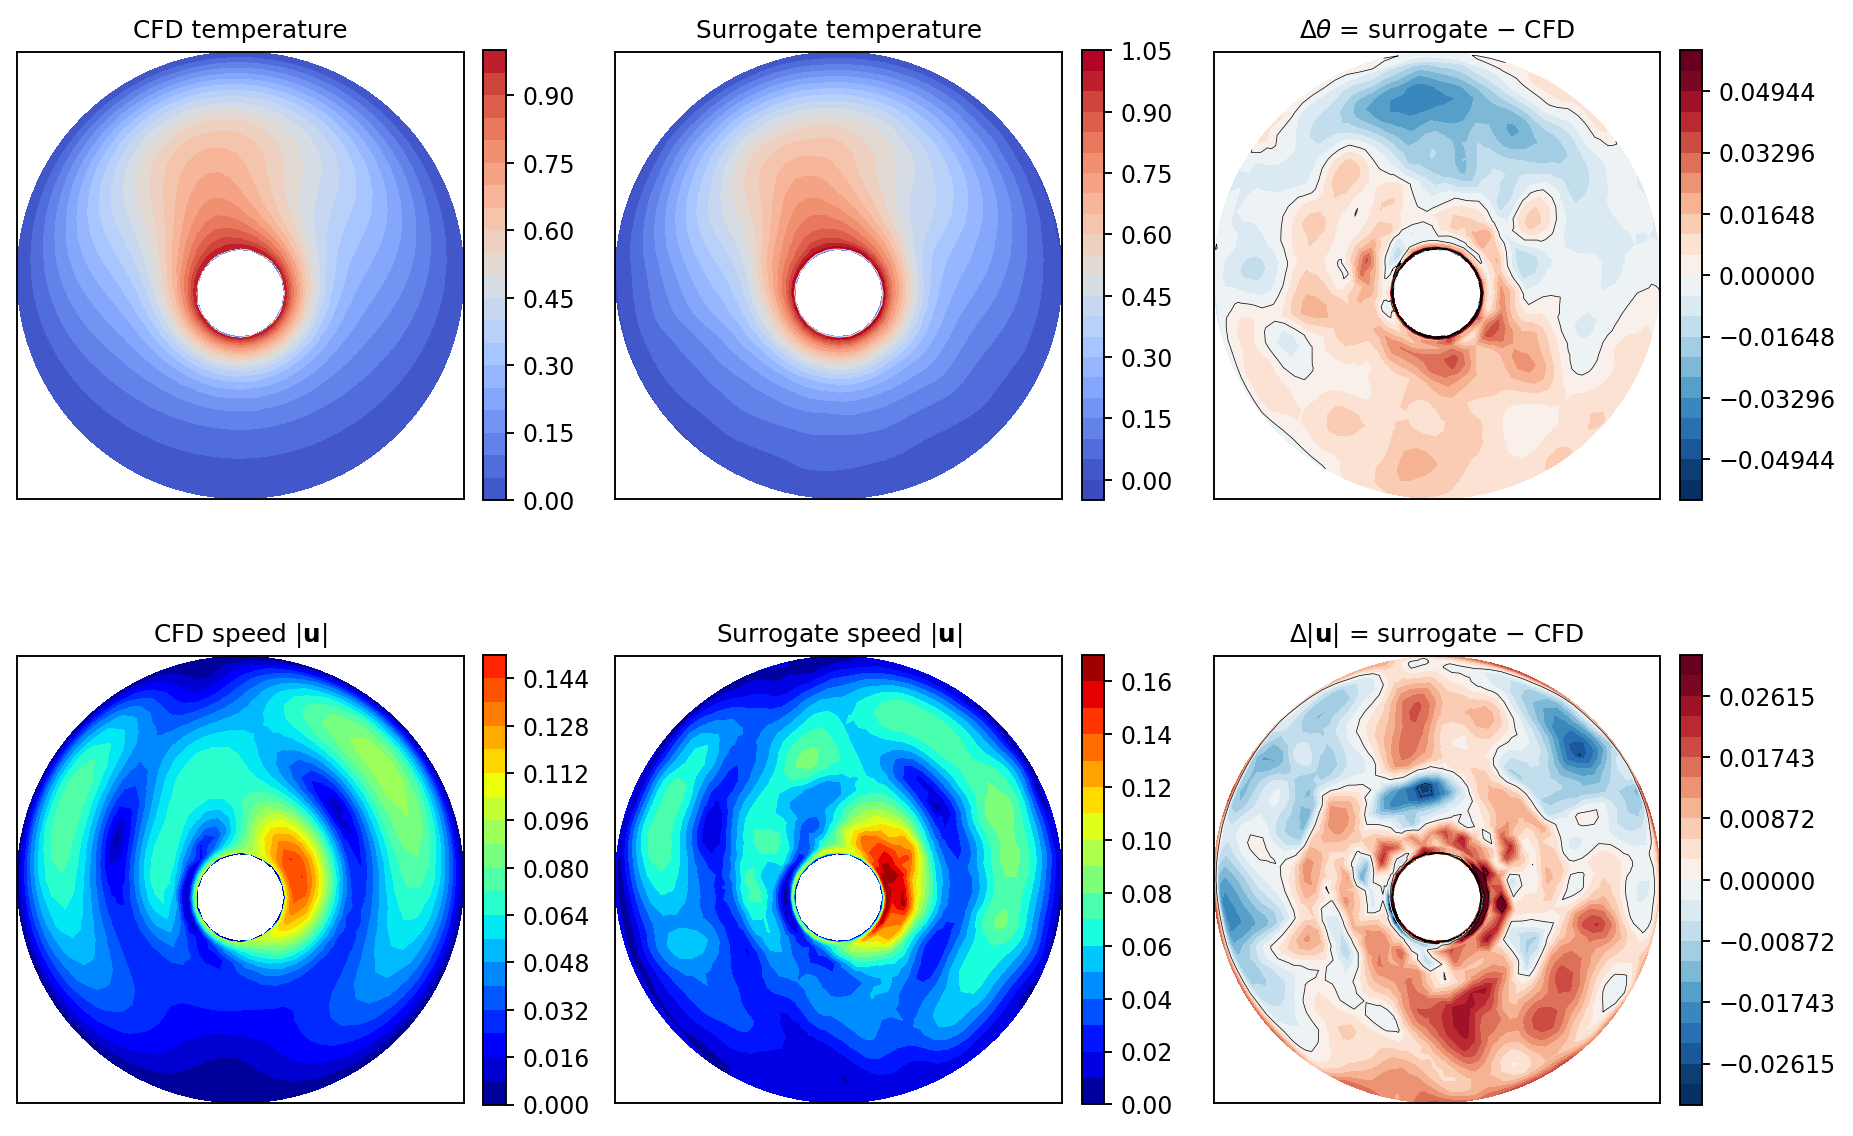
\includegraphics[width=\textwidth]{figures/fig_oor_field.png}
\caption{Out-of-range field validation: CFD versus per-node MLP surrogate prediction at $Re=500$, $Ri=0.2$ (absent from the training grid; the scalar surrogate's largest-error blind-test point), held-out geometry $R^\ast=0.2$, $\varepsilon=0.04$. Top: temperature. Bottom: velocity magnitude. Right column: signed difference (surrogate minus CFD, dimensionless, both fields already non-dimensional) with contour lines; the color scale is clipped at the 98th percentile of the absolute difference.}
\label{fig:oor-field}
\end{figure}

\subsubsection{Uncertainty Quantification}
\label{subsec:field_uq}

A five-member deep ensemble of the winning per-node MLP architecture was evaluated on the same held-out-geometry test split. Ensembling improved point accuracy slightly over the single-model baseline ($R^2 = 0.973/0.969/0.974$ for temperature, $u$, $v$, versus $0.966/0.962/0.967$ for the single model). Calibration, the fraction of true values within the ensemble's 95\% predictive interval, was $92.8\%$ for temperature, $92.2\%$ for $u$, and $90.2\%$ for $v$: modestly under-covered relative to the 95\% target, but markedly better behaved than the scalar surrogate's true-out-of-sample calibration collapse reported above. This is not a directly comparable test, however: this calibration check generalizes across unseen geometries while every $(Re,Ri)$ value within those geometries was part of the original training grid, whereas the single out-of-range field case described above tests an unseen $(Re,Ri)$ combination but was not repeated across a full ensemble. A systematic, ensemble-based out-of-range calibration check for the field surrogate, directly matched to the scalar surrogate's protocol, remains an item for future work.

\subsection{Limitations}
\label{sec:limitations}

Several limitations should be considered when interpreting these results. First, the highest achieved Rayleigh number in this study, $Ra \approx 7.1\times10^6$ (at $Re=1000$, $Ri=10$), sits well beyond where independent numerical work on a related, though not identical, geometry reports a failure to reach a steady state~\cite{Pranowo2024}. All 5,460 production simulations and all eighteen true out-of-sample checks satisfied the adaptive convergence criterion described above; a converged solution is not by itself proof of physical steadiness, so this concern remains open pending an explicit time-accurate check at the highest-$Ra$ corner of the sweep. Second, grid independence was demonstrated at a single representative operating point rather than across the full parameter space; extending this to additional points, particularly at the highest Reynolds and Richardson numbers, would strengthen this claim further. Third, the true out-of-sample test for the scalar surrogate covered eighteen points across six geometries, and the equivalent field-surrogate check covered a single point; a larger and more systematically designed out-of-sample test set for both surrogates would further strengthen the accuracy claims made here. Relatedly, the scalar surrogate's two robustness checks each test a single generalization axis at a time (LOGO cross-validation holds out geometries at in-grid operating conditions; the true out-of-sample test holds out operating conditions at in-grid geometries), not both simultaneously; a combined held-out-geometry-and-held-out-condition test, as performed once for the field surrogate, remains for future work. Fourth, the true out-of-sample error above concentrates specifically where the Reynolds-number sampling grid is coarsest in absolute terms, despite being log-spaced for even coverage in relative terms (Section~\ref{subsec:oos}); a sampling design dense in absolute, not only relative, terms at the high-$Re$ end would likely reduce this specific source of error and is a concrete target for future dataset extensions.
